%this is a comment
%this is a latex live doc bcz rush bcz merges are too much work rn
%write raw latex here and we can build and fix it later
%bcz html doesnt care lol
\documentclass[a4paper,10pt]{article}
\usepackage[utf8x]{inputenc} 
\usepackage{graphicx}
\usepackage{float}

%opening
\title{Group 12 Project Proposal and Requirements Document}
\author{Eric Momper, Peter Lomason, John Barber}
\setlength{\parindent}{0pt}
\begin{document}
	
	\maketitle
	
	\pagebreak
	\tableofcontents
	\pagebreak
	
	\section{Introduction}
	Our Project is intended to be a psychological theraputic tool that helps patients through simulation in Virtual Reality.
	Many of the new up and coming Virtual Reality devices look very promising at providing better and more realistic immersion and simulation for users at a lower cost than ever before. We aim to bring psychological tools to the home of the average user. This will allow those seeking certain therapies or treatments to perform them more often since such services often require high diligence and repetition to produce results.
	\\
	\paragraph{A few of these devices include:}
	\begin{itemize}
		\item Occulus Rift, Occulus Touch
		\item HTC Vive
		\item Samsung Gear VR
		\item Google Cardboard
		\item Microsoft Hololens
	\end{itemize}
	
	\paragraph{ Some of our project ideas are related to the following:}
	\begin{itemize}
		\item ​Immersion Therapy for phobias, dysphorias, or PTSD (Virtual or Augmented Reality)
		\item Therapy for burn victims, phantom pain for amputees,  (Virtual Reality)
		\item Creating a calm environment for  anxiety disorders, or autism (Virtual Reality)
		\item Creating a drawing art therapy tool that allows for creativity in 3D space (Virtual or Augmented Reality)
	\end{itemize}
	
	
	\paragraph{Project Direction} ~\\ We are currently contacting faculty in the psychology department for collaboration or guidance on opportunities to use our project for helping their patients or for their research.
	\paragraph{Integration} ~\\ Our project will be created in Unity, Unnreal Engine, or written with a C++ OpenGL/ DirectX SDK wrapper, depending on the direction of our design, and the VR device we have available. It will most likely be windows exclusive as many VR devices are dropping Linux and OSX support unless we can find some options that will provide cross platform systems, which is said to be available in the near future for some platforms but not currently finished.  
	
	\pagebreak
	
	\section{Status of Virtual Reality in Psychology}
	The first use of Virtual Reality therapy in Psychology was in 1995 by psychologist Barbara Rothbaum and computer scientist Larry Hodges. T
	hey found that virtual reality therapy could help patients overcome phobias such as arachnophobia or a fear of heights. Since then many others 
	have used virtual reality as a tool in psychology. The main use of virtual reality in psychology is a form of treatment called Exposure Therapy. 
	This type of treatment can be used to address psychological issues such as Autism spectrum disorder, Obsessive Compulsive Disorder, various phobias, 
	post-traumatic stress disorder, and phantom limb pain. The greatest issue facing treatment with Exposure Therapy is that it requires a high level of diligence and
	repetition. Typically patients cannot make time for appointments as frequently as is required.
	
	\subsection{Exposure Therapy}
	\subsection{Immersion Therapy}
	AR
	\subsection{Pain Treatment}
	AR, VR
	\subsection{Creating a Calming Environment}
	AR
	\subsection{Art Therapy}
	AR, VR
	\pagebreak
	
	\section{Team Member Motivations}
	\subsection{Eric Momper}
	My personal motivation for this project is that it is similar to some of the programming I do on my internship (OpenGL and OpenCL image GPGPU processing).
	I also have taken computer graphics with Professor Leinicker and I am currently taking robot vision with Doctor Lobo. This project will be very interesting to me as  
	I will be working with new technologies and programming on a new type of 3D graphics platform. I am also looking forward to studying the psychological benefits
	of Virtual Reality on patients with various disorders.  
	
	\subsection{John Barber}
	This project was my idea, and combines two different fields, virtual reality and psychology.  In the same way, i'm interested in both 
	sides seperately, and really hopeful about how they can be combined.  Virtual Reality is exciting to me as a game designer, 
	and one of my closest friends went to work for Emblematic Group, and we've been comparing notes on the future of virtual reality since.  
	However, I also have seen a number of my friends struggle with psychological issues, and have been hoping to find a way to use my Computer 
	Science degree after I graduate to help people.  This is an opportunity to not only accomplish that now, pushing the field forward and finding 
	new ways to use it for people, but also to train myself and find opportunities and connections for the future.
	\subsection{Peter Lomason}
	My interest in this project mainly comes from past experience with virtual reality tools. I used to own an Oculus Rift DK1 and at the time I had it, 
	I was not knowledgeable enough to develop for it. Now I would like to apply what I have learned at UCF to virtual reality development. I eventually want to be
	a video game developer and virtual reality for psychology shares many aspects with that. Being able to program an environment, objects, and interactions is very
	interesting to me and this project will allow me to strengthen my ability to do these tasks.
	\pagebreak
	\section{Goals and Objectives}
	Design an environment in Virtual Reality that can be customized and used to help a variety of psychological conditions, and further psychology research, that is accessible to the typical user so they may conduct their own treatment on their own time.
	\begin{itemize}
		\item Increase our understanding of psychology principals \& problems and how virtual reality can help certain conditions.
		\item Find a platform that we can develop on, that creates a high quality virtual reality experience, and is reasonably up to date with modern graphics. Currently our best candidate is the Unity Engine.
		\item Integrate some level of user intractability in the created virtual environments. 
		\item Procedural generation of environments with parameters that can be customized by the user. 
		\item Include pre-constructed environments similar to current treatment strategies in the VR Psychology industry.
	\end{itemize}
	
	\section{Function}
	Make a customizable environment which includes settings for some or all of following:
	\subsection{Therapeutic Art Deign Environment}
	This calming art suite allows users to relax and design art in a creative 
	\begin{itemize}
		\item The user can use hand controls or a controller to draw colors and shapes in a 3D space around them. 
		\item This can be used on a variety of platforms including Ouculus Rift, HTC Vive, and PS VR.
	\end{itemize}   
	\subsection{Music Visualization}
	This module would be related to music visualization. 
	\begin{itemize}
		\item The different sound or frequencies that could be visualized via colors and waves that are around the user as music is playing in real time.
		\item The user can interact with these sounds in some way possible a puzzle.(see auditorium game)
	\end{itemize}   
	\subsection{A Virtual 3D World Targeted at a Specific Treatment}
	This module would be a variety of 3D world that the user could move in and interact with. 
	\begin{itemize}
		\item The user can use hand controls or a controller to draw colors and shapes in a 3D space around them. 
		\item This can be used on a variety of platforms including Ouculus Rift, HTC Vive, and PS VR.
	\end{itemize}
	
	\section{Broader Impacts}
	%Broad implications and impact on society (impact on underrepresented? within STEM and or society as a whole? disabled? non-profit orgs? environment? diversity? increased participation in STEM or workforce? public engagement in STEM? improve national security? enhanced infrastructure? improved education?)
	
	%qualitative, avoid numbers, conceptual discussion specific to project. example descriptions "“lightweight, portable, programmable, low cost, flexible, high resolution, scalable, low power, accurate, mobile, peer-to-peer, autonomic”
	
	Our project would have an impact on the field of psychology as it relates to certain emotional disorders or struggles and the deployment of self-administered therapy for those disorders. It would not only be relevant to those diagnosed with a psychological condition, but also those seeking stress relief or a unique environment to immerse themselves in. By bringing treatment therapies to the end user in their own home and allowing them to perform therapy at their leisure we will have an impact on many people seeking these services who may not have the time to schedule appointments or those who simply won't try due to the stigma surrounding therapy.
	\pagebreak
	\section{Requirements}
	\subsection{Functinal Requirements}
	\begin{enumerate}
		\item Project will create some 3D environment that the user can can see and interact with in 3D space.
		\item The project will must have modules that provide some kind of psychological treatment for end users at home.
		\item The prebuilt environments will allow users to modify and save the worlds and change or redesign them.
		\item There will be some sort of user controls allow the user to interact with menus and the environment.
	\end{enumerate}
	
	\subsection{Performance Requirements}
	\begin{enumerate}
		\item User must have a computer that runs windows (for now) and has sufficient GPU and other system specs to run a VR headset.
		\item The VR environment must run at least 30 FPS on an appropiate platform.
		\item User control interactions must be responsive and fluid (reasonable interaction responses).
	\end{enumerate}
	\subsection{Users and Human Factors Requirements}
	\begin{enumerate}
		\item The dialogs and menus must be easy to see and use.
		\item Some user interactions must be desktop based to be simpler (ex file menus).
		\item The models in the app must be decent quality.
	\end{enumerate}
	
    \pagebreak
    \section{Diagrams}
	\subsection{Block Diagrams:}
	\begin{figure}[ht!]
	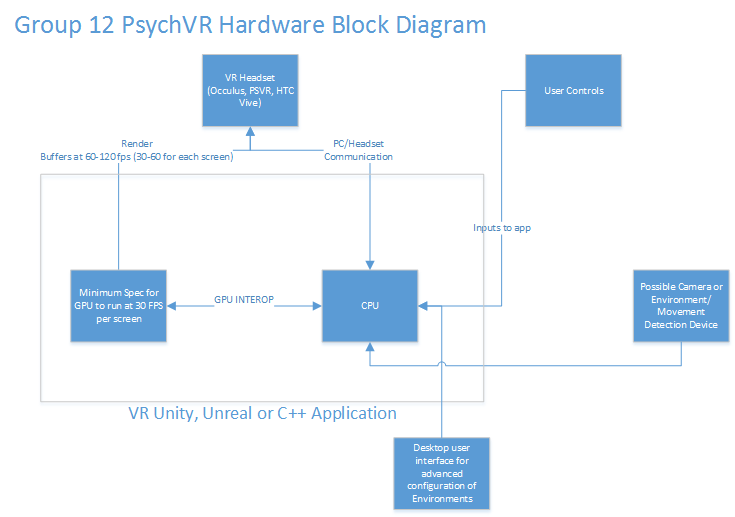
\includegraphics[width=\linewidth]{HardwareConfig.png}
	\caption{Hardware Block Diagram}
	%to ref fig number
	%Figure \ref{fig:block1} shows our blockDiagram.
	\label{fig:hblock}
	\end{figure}
	\begin{figure}[ht!]
	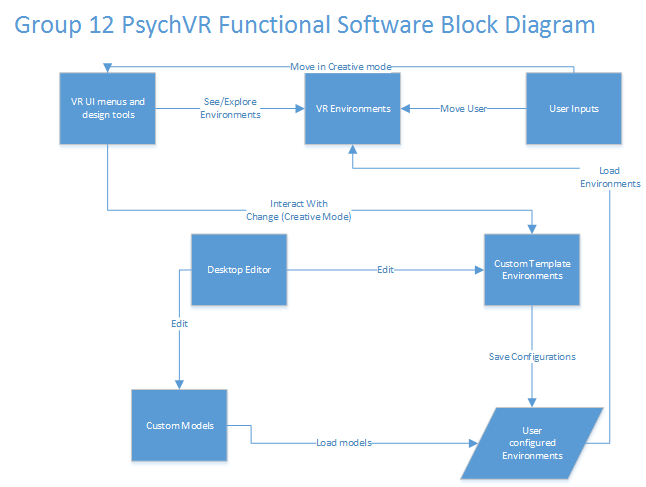
\includegraphics[width=\linewidth]{SoftwareConfig.png}
	\caption{Software Block Diagram}
	%to ref fig number
	%Figure \ref{fig:block1} shows our blockDiagram.
	\label{fig:sblock}
	\end{figure}
	\pagebreak
	\subsection{Schedules:}
	\begin{figure}[h!]
	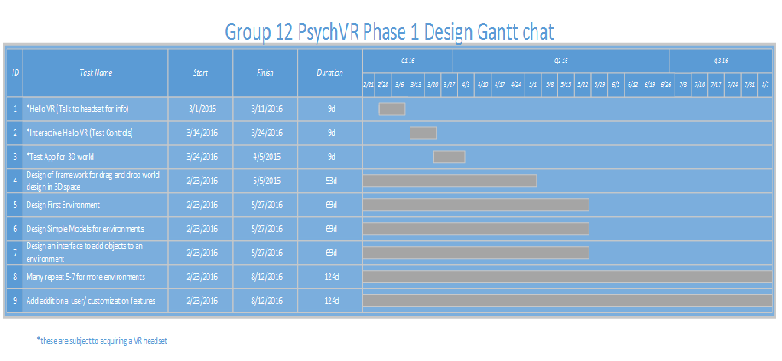
\includegraphics[width=\linewidth]{scheduleSR.png}
	\caption{Prototype Phase Gantt Chart:}
	%to ref fig number
	%Figure \ref{fig:block1} shows our blockDiagram.
	\label{fig:pchart}
	\end{figure}
	\pagebreak
	
	\subsection{Specs}
	%some design reqs go here
	
	%project block diagrams - gantt chart goes here
	%prototype illustration?
	
	
	
	%\begin{enumerate}
	%	\item The name of the Group member administratively responsible for the block.
	%	\item Block name, which is descriptive of its function.
	%	\item Block status:
	%	\begin{enumerate}
	%		\item To be acquired – meaning the block will be purchased or donated
	%		\item Acquired – block has been donated or purchased
	%		\item Research – block design approach is being investigated
	%		\item Design – block is currently being designed
	%		\item Prototype – block is currently being prototyped
	%		\item Completed – block design is a finished prototype
	%	\end{enumerate}
	%	\item Name each input and output associated with each block
	%	\item Diagram Legend. The legend should expand all acronyms and describe all named entities in the block diagram by giving brief definitions.
	%\end{enumerate}
	%Include any additional information that would increase the understanding of the block diagram. The use of identifier grouping and color may be helpful. 
	\section{Budget and Financing}
	%software licensing costs, cloud based service costs, code repo's, graphic design costs
	\section{Milestones}
\end{document}
